\chapter{The analytical simulators}
\label{ch:sims}

\section{Framework}
Each simulator in \file{sims.js} is a plain object: a list of \texttt{inputs} (sliders and selectors) and a function \texttt{compute(v)} returning a status banner, readouts, charts and the governing equations. The framework draws the controls, calls \texttt{compute} on every change, and adds an A/B comparison (a saved state drawn dotted), CSV/SVG/lab-report export, URL routing (\texttt{\#beam}) and light/dark themes. \texttt{registerModule} lets another file add a tab (the FEM tab does this). Mohr's circle was described in Chapter~\ref{ch:stress}; the other eight are summarised below.

\section{Beams}
\physics{Equilibrium gives $dV/dx=-w$ and $dM/dx=V$; Euler--Bernoulli theory gives $v''=M/EI$, $\sigma=My/I$ and $\tau=VQ/(Ib)$. Timoshenko theory adds a shear deflection $V/(k_sGA)$, important only for short deep beams.}
\code{Reactions follow from statics (simply supported or cantilever; point load, UDL and moment by superposition). $V$ and $M$ are evaluated at 401 points, $M/EI$ is integrated twice with the trapezoidal rule, and the boundary conditions are then imposed. $Q(y)$ is integrated numerically, so rectangle, circle and tube need no separate formulas.}
@@CODE sims.js|const slope0 = cumtrapz|10@@

\section{Shaft torsion and axial loading}
\physics{\textbf{Torsion:} plane sections rotate rigidly, so $\tau(r)=Tr/J$ and $\phi=TL/GJ$ with $J=\pi(D^4-d^4)/32$ and $G=E/2(1+\nu)$. The simulator also draws a 3D shaft whose end face is coloured by $\tau\propto r$.
\textbf{Axial:} for a segmented bar the internal forces come from cuts and each segment stretches by $N_iL_i/(EA_i)+\alpha\Delta T L_i$. With both ends fixed the wall reaction $X$ is the redundant, found from zero total elongation:
\begin{equation}
X=-\frac{\sum_iN_i^{\text{free}}L_i/(EA_i)+\alpha\Delta T\sum_iL_i}{\sum_iL_i/(EA_i)} .
\end{equation}
A heated fixed bar with no load gives $\sigma=-E\alpha\Delta T$ ($-120$~MPa for steel at $50^\circ$C).}

\section{Pressure vessels and thermal stress}
\physics{\textbf{Vessels:} thin wall $\sigma_\theta=pr/t$ (cylinder) or $pr/2t$ (sphere). Thick wall uses the Lam\'e solution, for a cylinder
\begin{equation}
\sigma_{r,\theta}=A\mp\frac{B}{r^2},\qquad A=\frac{p_ia^2-p_ob^2}{b^2-a^2},\quad B=\frac{(p_i-p_o)a^2b^2}{b^2-a^2},
\end{equation}
and the analogous $1/r^3$ form for a sphere. The thin-wall error against Lam\'e is reported.
\textbf{Thermal:} a temperature change $\Delta T$ fully restrained in one, two or three directions gives $\sigma=-E\alpha\Delta T$, $-E\alpha\Delta T/(1-\nu)$ or $-E\alpha\Delta T/(1-2\nu)$; a partial restraint scales the stress.}

\section{Failure theories and energy methods}
\physics{\textbf{Failure:} Rankine ($\max|\sigma_i|$), St Venant ($\epsilon_1E$), Tresca ($\sigma_1-\sigma_3$) and von Mises are each compared with the strength $\sigma_{cr}$; the theory with the lowest safety factor governs. Their envelopes in the $(\sigma_1,\sigma_2)$ plane (square, skewed square, hexagon, ellipse) are drawn with the current state.
\textbf{Energy:} the strain energy $U$ of a bar, shaft or beam (bending and shear) is evaluated in closed form; Castigliano's theorem $\delta=\partial U/\partial P$ is checked by \emph{numerical} differentiation against the closed-form displacement, and Maxwell--Betti reciprocity is checked on a simply supported beam.}

\section{Column buckling}
\physics{Euler's load is $P_{cr}=\pi^2EI/(KL)^2$ with $K=1,\,0.699,\,0.5,\,2$ for the four end conditions and $I$ the weak-axis value. It holds only for slenderness $\lambda=KL/r>\lambda_c=\pi\sqrt{E/\sigma_y}$; shorter columns use the Johnson parabola $\sigma_{cr}=\sigma_y[1-\sigma_y\lambda^2/(4\pi^2E)]$, which meets Euler's curve at $\lambda_c$.}

\chapter{The finite element method}
\label{ch:fem}

\section{Method and implementation}
The half-space solution is exact only for an infinite body and the simulators only for simple members. The finite element method solves the same equations on a body of any shape:
\begin{enumerate}[nosep]
\item mesh the body into elements joined at nodes, whose displacements are the unknowns;
\item interpolate inside each element, $\mathbf u=\sum_iN_i\mathbf u_i$, so that $\tens\epsilon=\mathbf B\mathbf u_e$ and $\tens\sigma=\mathbf D\tens\epsilon$;
\item form $\mathbf k_e=\int\mathbf B^T\mathbf D\mathbf B\,dV$ by Gauss quadrature and assemble the global $\mathbf K$;
\item remove supported degrees of freedom, solve $\mathbf K\mathbf u=\mathbf f$, and recover stresses and the reactions $\mathbf R=\mathbf K\mathbf u-\mathbf f$.
\end{enumerate}
@@CODE fem.py|def solve_system|9@@

\section{Elements and test problems}
\begin{itemize}[leftmargin=*]
\item \textbf{Tapered bar} (2-node elements): exact solution $u=\frac{P}{Em}\ln\frac{A(x)}{A_0}$; the FEM converges as $h^2$.
\item \textbf{Beam} (Hermite cubic, deflection and slope per node): nodal deflections are exact for any mesh, because the cubic solves $EIv''''=0$ between loads.
\item \textbf{Plane stress} with $\mathbf D=\frac{E}{1-\nu^2}\left[\begin{smallmatrix}1&\nu&0\\\nu&1&0\\0&0&(1-\nu)/2\end{smallmatrix}\right]$: the constant-strain triangle (CST) and the four-node quadrilateral (Q4, $2\times2$ Gauss points, stresses extrapolated to nodes and averaged). Two problems are solved: a cantilever under end shear (compared with Euler--Bernoulli and Timoshenko), and a quarter plate with a hole in tension, compared with Kirsch's $K_t=3$~\cite{kirsch}.
\end{itemize}

\section{The three-dimensional block}
\label{sec:block}
\physics{A cuboid with a square patch pressure $q$ on its top is meshed (one quarter, using symmetry) with 8-node bricks. The sides and unloaded top are free: the weak form makes their traction zero automatically, which is exactly what the half-space solution cannot do. The reference is Newmark's solution for the vertical stress under a rectangular patch~\cite{newmark}.}
\code{All bricks are identical, so one $24\times24$ stiffness matrix is reused. The system is solved \emph{matrix-free} by Jacobi-preconditioned conjugate gradients: $\mathbf K\mathbf x$ is assembled brick by brick by gather, multiply and scatter (\texttt{np.bincount}), so $\mathbf K$ is never formed.}
@@CODE fem3d.py|def cg|13@@

\textbf{User interface.} \file{fem.js} sends the inputs of the five problems to \texttt{POST /api/fem/solve} and draws the returned mesh coloured by stress, the charts, a FEM-versus-reference table and a panel describing what the solver did with the current numbers (Figure~\ref{fig:femui}).

\begin{figure}[ht]
\centering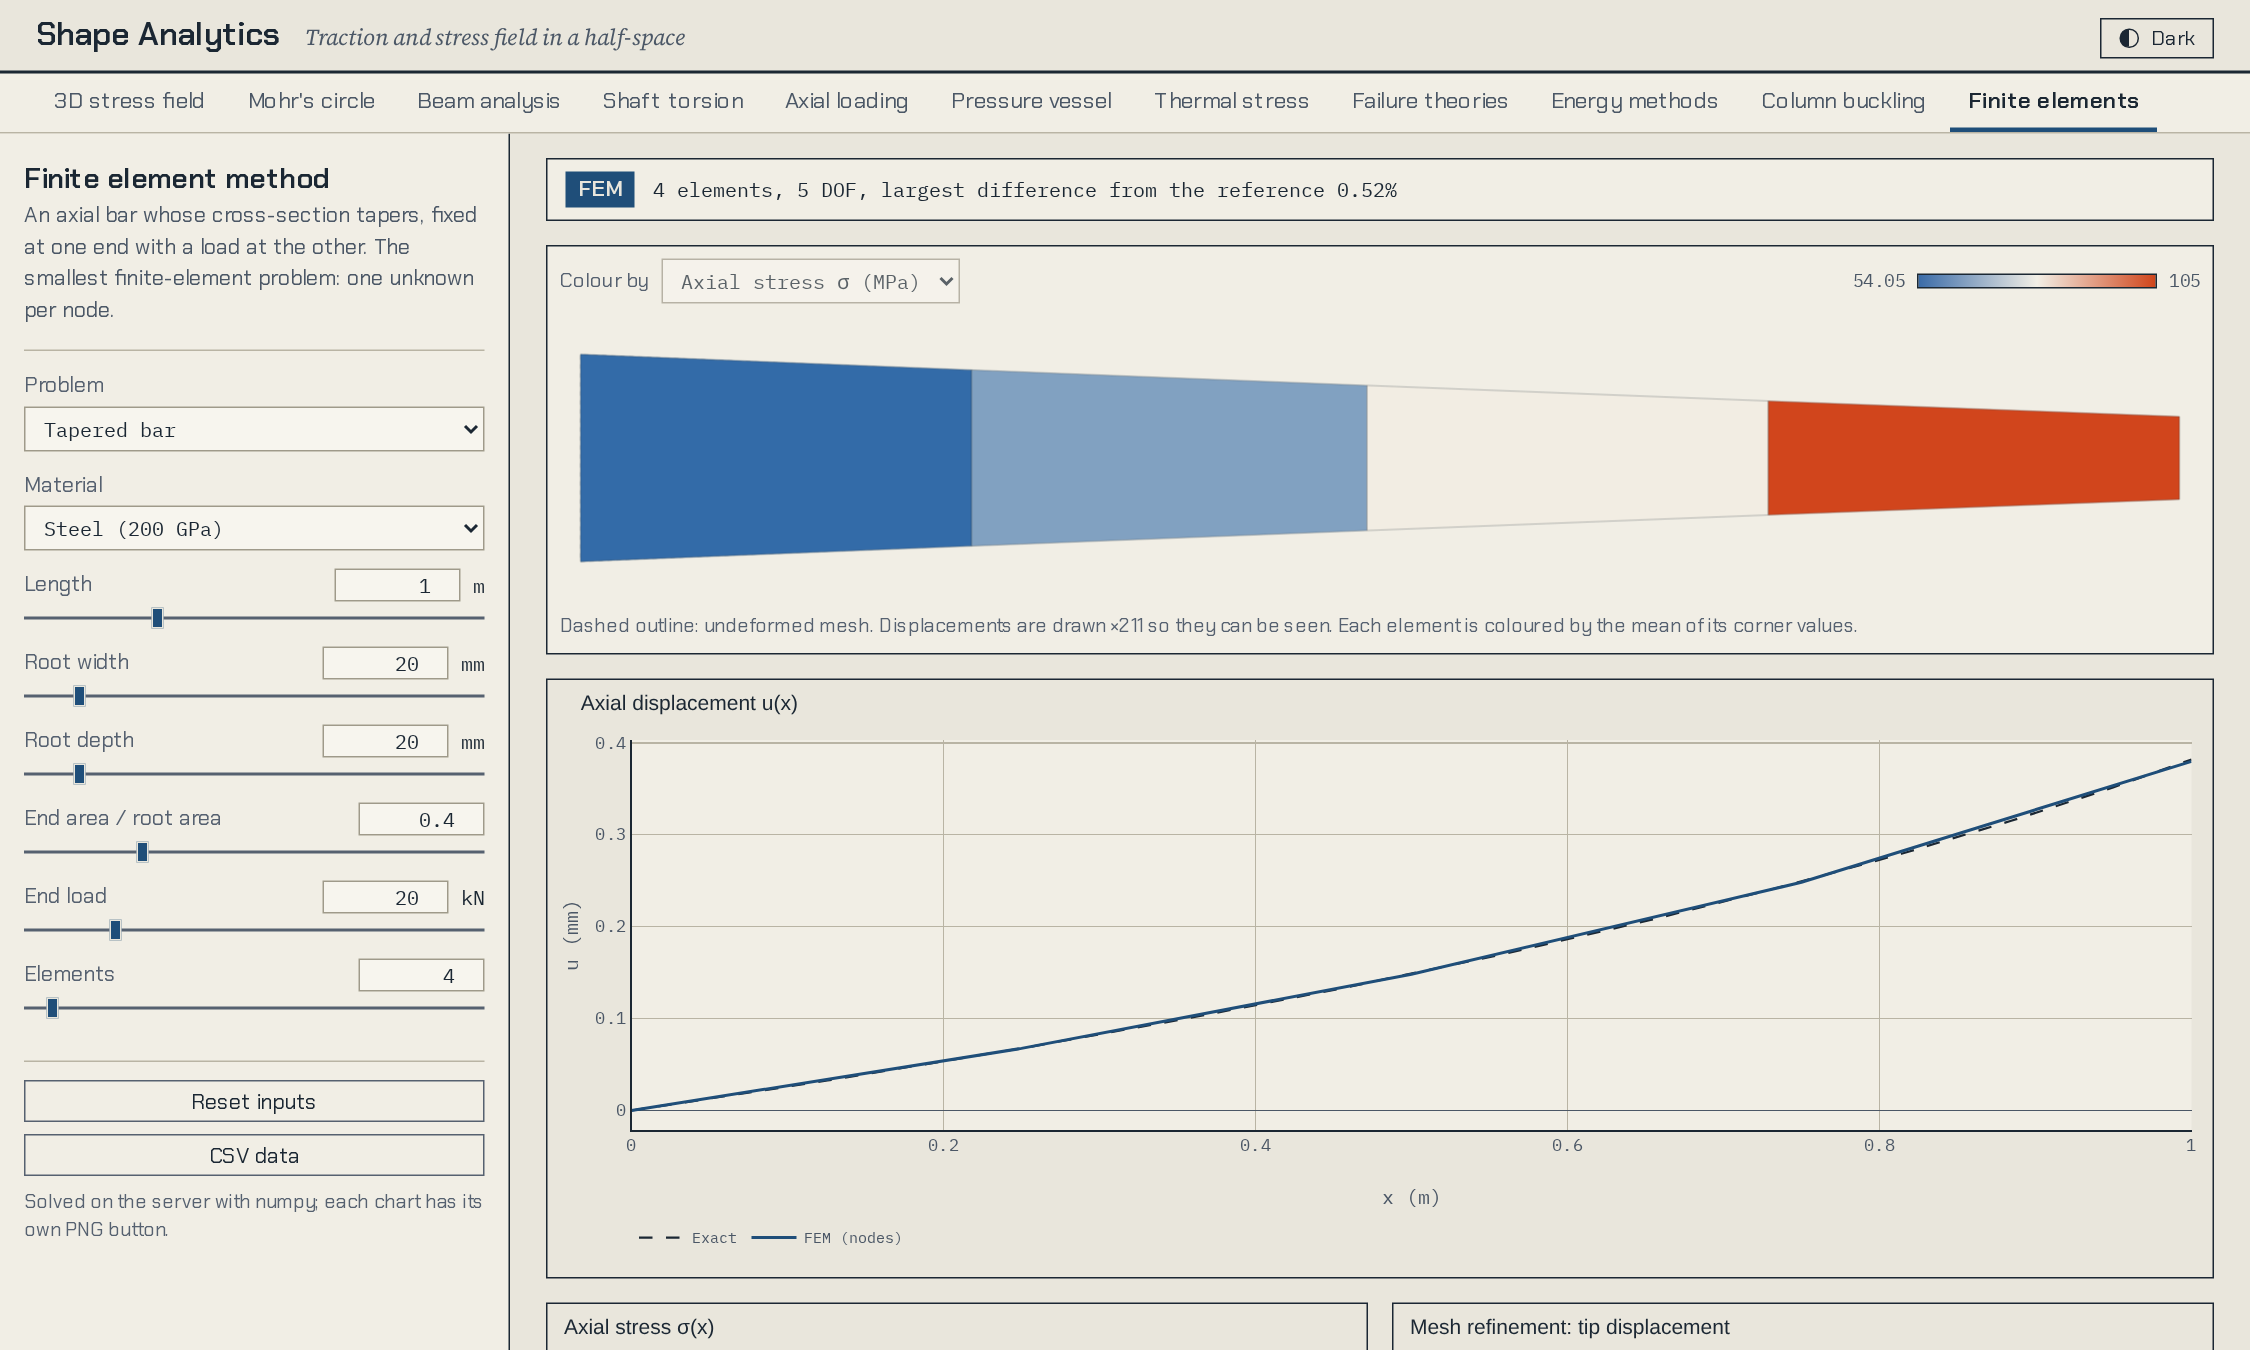
\includegraphics[width=0.9\linewidth]{../figures/ui_fem.png}
\caption{The finite element tab for the tapered bar: mesh coloured by axial stress and displacement against the exact solution. With four elements the largest error is $0.52\%$.}\label{fig:femui}
\end{figure}
